
%
% raspberry p3 spec: https://www.raspberrypi.org/magpi/raspberry-pi-3-specs-benchmarks/

\section{Embedded Computing Platform Comparison}\label{sec:comparison}

In this section, we compare three computing platforms---the Raspberry
Pi 3, the Intel UP~\footnote{http://www.up-board.org/up/} and NVIDIA
Jetson
TX2~\footnote{http://www.nvidia.com/object/embedded-systems-dev-kits-modules.html}---from
the point of view of supporting vision-based end-to-end deep learning
based autonomous vehicles.

Table~\ref{tbl:platforms}
  
Our basic approach is to use the same DeepPicar's software, and repeat
the experiments in Section~\ref{sec:evaluation} on each hardware
platform and compare the results.



\begin{figure}[h]
  \centering
  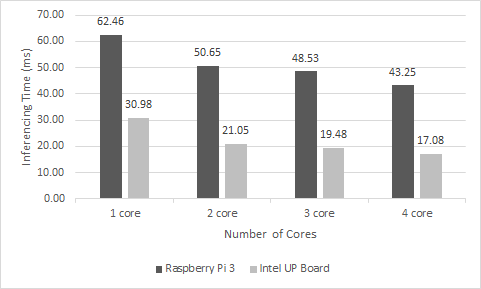
\includegraphics[width=.5\textwidth]{figs/system_multicore}
  \caption{Inferencing time across platforms based on number of cores used.}
  \label{fig:sys_core}
\end{figure}

The results of the multicore tests can be seen in Figure~\ref{fig:sys_core}. It was found that the 
Intel UP Board performed better in all experiments. On average, it was able to perform inferencing 
operations, at least, twice as fast as the Raspberry Pi 3. As a result, the UP Board was able to 
satisfy the 50 ms WCET by a very clear margin (in the worst case, it would still meet it by $\sim$20 
ms), and, thus, demonstrates that it is more capable of autonomous driving than the Raspberry Pi 3.

The Intel UP Board also performed better in the multimodel tests, as is shown in 
Figure~\ref{fig:sys_model}. Once again, the UP was able to complete inferecing operations in half the 
time when compared to the Pi. Furthermore, the Intel UP Board was capable of satisfying the 50 ms 
WCET, while the Raspberry Pi 3 was unable to do so. As such, the Intel UP Board displays greater 
potential for the simultaneous execution of multiple models during self-driving operation, while the 
Raspberry Pi 3 would struggle to do so.

\begin{figure}[h]
  \centering
  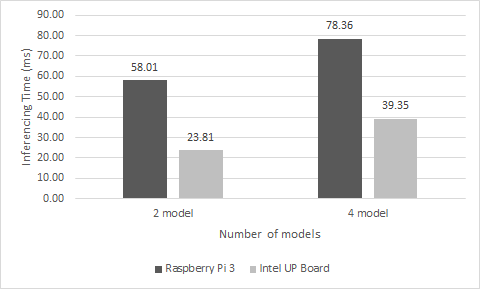
\includegraphics[width=.5\textwidth]{figs/system_multimodel}
  \caption{Inferencing time across platforms based on number of models run concurrently.}
  \label{fig:sys_model}
\end{figure}

Finally, we examined if the performance of the Intel UP Board and Tegra TX2 would be affected by the 
addition of the synthetic benchmarks. As summarized in Figure~\ref{fig;sys_bench}, the Intel UP Board 
did experience a change in its inferencing times, but the increase was not as drastic as is seen by 
the Raspberry Pi 3. in the worst case, the Intel UP Board produced times that were over two times as 
large, whereas the Raspberry Pi 3 output times that were around 10 times greater. The Intel UP Board 
was successful in completing inferencing operations in under 50 ms when benchmarks were run on a 
maximum of 2 cores, while the Raspberry Pi 3 failed to do so when any benchmark was introduced. As 
such, it can be concluded that the Intel UP Board would be more capable of running computationally 
heavy processes during autonomous driving, and that the Pi wouldn't be able to do the same.

\begin{figure}[h]
  \centering
  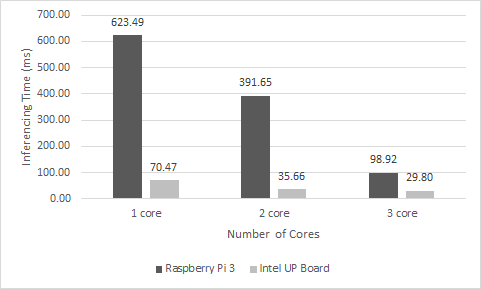
\includegraphics[width=.5\textwidth]{figs/system_benchmark}
  \caption{Inferencing time across platforms based on number of cores used.}
  \label{fig:sys_bench}
\end{figure} 

In the comparison of the real-time capabilities of three embedded computing platforms, we found that 
the Raspberry Pi 3 performed the worst. When compared to the Intel UP Board, inferencing on the Pi 
took twice as long across all multicore and multimodel experiments. The difference was even more 
noticeable in the the addition of computationally heavy synthetic benchmarks that had a much more 
dire effect on the Pi.



